\documentclass[conference]{IEEEtran}

% para correr / compilar 
% pdflatex main.tex
% bibtex main
% pdflatex main.tex
% pdflatex main.tex
% 

\usepackage[spanish]{babel}
\usepackage{amsmath,amssymb,amsfonts,amsthm}
\usepackage[utf8]{inputenc} % Caracteres en Español (Acentos, ñs)
\usepackage{csquotes}
\usepackage{graphicx}
\usepackage{url} % ACENTOS
\usepackage{hyperref} % Referencias
\usepackage{subfig}
\usepackage{lipsum}
\usepackage{balance} 
\usepackage{etoolbox}
\usepackage{datetime}
\usepackage{float}
\makeatletter
\patchcmd{\frontmatter@RRAP@format}{(}{}{}{}
\patchcmd{\frontmatter@RRAP@format}{)}{}{}{}
\makeatother	

\usepackage[backend=bibtex,sorting=none]{biblatex}
\setcounter{biburllcpenalty}{7000}
\setcounter{biburlucpenalty}{8000}
\addbibresource{references.bib}

% fecha
\usepackage{datetime}
\newdateformat{specialdate}{
    \twodigit{\THEDAY}-\twodigit{\THEMONTH}-\THEYEAR
}
\date{\specialdate\today}

% la sentencia \burl en las citas... 
\usepackage[hyphenbreaks]{breakurl}
\renewcommand\spanishtablename{Tabla}
\renewcommand\spanishfigurename{Figura}


\begin{document}
% Definitions
\newcommand{\breite}{0.9} %  for twocolumn
\newcommand{\RelacionFiguradoscolumnas}{0.9}
\newcommand{\RelacionFiguradoscolumnasPuntoCinco}{0.45}

%Title of paper
\title{Proyecto en Equipo U1 \\ Detección de Piedras en los Frijoles}

% Trabajo Individual
\author{
    \IEEEauthorblockN{
        Ricardo Emmanuel Uriegas Ibarra\IEEEauthorrefmark{1}
    }
    \IEEEauthorblockN{
        Hector Israel Cruz Resendez\IEEEauthorrefmark{1}
    }
    % En caso de trabajos en equipo, poner a todos los autores 
    % en estricto ORDEN ALFABETICO
    %\author{\IEEEauthorblockN{Michael Shell\IEEEauthorrefmark{1},
    %Homer Simpson\IEEEauthorrefmark{1}}
    \IEEEauthorblockA{
        \IEEEauthorrefmark{1}Ingeniería en Tecnologías de la Información\\
        Universidad Politécnica de Victoria
    }
}

\maketitle

%%%%%%%%%%%%%%%%%%%%%%%%%%%%%%%%%%%%%%%%%%%%%%%%%%%%%%%%%%%%%%%%%%%%%%%
\begin{abstract} 
    
\end{abstract}

%%%%%%%%%%%%%%%%%%%%%%%%%%%%%%%%%%%%%%%%%%%%%%%%%%%%%%%%%%%%%%%%%%%%%%%
\section{Introducción}
    % 

%%%%%%%%%%%%%%%%%%%%%%%%%%%%%%%%%%%%%%%%%%%%%%%%%%%%%%%%%%%%%%%%%%%%%%%
\section{Desarrollo Experimental}
    En este trabajo se desarrollo un sistema capaz de detectar piedras en los frijoles dada una foto (sin usar ningún tipo de red neuronal). Para ello se utiliza la librería OpenCV\cite{opencv} en Python\cite{python}, en combinación de la librería PyQt6\cite{pyqt6} para la interfaz gráfica.
    Debido a las limitaciones de tiempo y recursos, se desarrolla el sistema solamente para 2 tipos de frijoles; pinto y negro. 

    \subsection{Características del Frijol}
    \subsubsection{Frijol Pinto}
    El frijol pinto tiene las siguientes características:
    \begin{enumerate}
        \item Frijol color cafe claro con manchas cafe oscuro.
        \item Las piedras que llegan a aparecer en este tipo de frijoles son color negro.
        \item Forma ovalada.
        \item Textura lisa.
    \end{enumerate}

    \subsubsection{Frijol Negro}
    El frijol negro tiene las siguientes características:
    \begin{enumerate}
        \item Color negro uniforme con un punto blanco en el hilum\cite{semillas}.
        \item Las piedras que llegan a aparecer en este tipo de frijoles son color gris claro (cercano al color hueso\cite{pantone}).
        \item Forma ovalada.
        \item Textura lisa.
    \end{enumerate}

    \subsection{Características de las Fotos}
    Para el desarrollo del proyecto es necesario conseguir un conjunto de pruebas que permitan verificar su correcto funcionamiento. Este conjunto de pruebas son fotos tomadas con un celular \textit{Iphone SE 2020}\cite{iphone} con dimesiones de $4,032 \times 3,024$ o $3,024 \times 4,032$, esto debido a que era el celular disponible por uno de los participantes del proyecto.

    Las imagen se tomaron con flash (tratando de evitar sombras que puedan interferir con el análisis de la imagen) y llevaran un fondo blanco o equivalente, mientras los frijoles se encontraran esparcidos a lo largo de la imagen, sin algun patron aparente.

    \subsection{Procesamiento previo al Análisis de la Imagen}
    Antes de analizar la imagen dada, se aplican varios filtros y transformaciones para tratar de facilitar la detección que se buscaba:

    \begin{itemize}
        \item Se redimensiona la imagen a un tamaño manejable para optimizar el procesamiento (esto debido al gran tamaño de las imágenes de con la que se probo).
        \item Se aplica un filtro de desenfoque Gaussiano (GaussianBlur) para reducir el ruido y suavizar la imagen\cite{gaussianblur}.
        \item Se convierte la imagen del espacio de color RGB a HSV\cite{rgbhsv} (Hue, Saturation, Value) para facilitar la segmentación por color (esto porque HSV es menos sensible a cambios de iluminación lo que ayuda a la detección de objetos).
        \item Se detecta si es frijol pinto o negro basado en el color dominante de la imagen.
        \item Se aplican máscaras de color específicas para cada tipo de frijol:
        \begin{itemize}
            \item Para frijol negro: Se filtran tonos oscuros cercanos al negro
            \item Para frijol pinto: Se filtran tonos café claro o cercanos al blanco hueso 
        \end{itemize}
        \item Se aplican operaciones morfológicas (erosión y dilatación) para eliminar ruido y mejorar la segmentación\cite{morfologico}.
    \end{itemize}

    \subsection{Segmentación de las Piedras}
    
    Para este momento gracias al preprocesamiento debería de ser sencillo segmentar; se realiza los siguientes pasos:
    \begin{enumerate}
        \item Se aplica un umbral adaptativo para separar los objetos del fondo.
        \item Se utiliza la función findContours para detectar los contornos de los objetos.
        \item Se filtran los contornos por área para eliminar objetos muy pequeños o muy grandes.
        \item Para cada contorno válido:
        \begin{itemize}
            \item Se calcula su área y perímetro 
            \item Se determina la forma aproximada usando approxPolyDP
            \item Se analiza el color promedio dentro del contorno para detectar si es frijol o piedra
        \end{itemize}
        \item Se clasifica como piedra si:
        \begin{itemize}
            \item Para frijoles negros:
            \begin{itemize}
                \item Área entre 1350 y 8000 píxeles
                \item Ratio de convexidad mayor a 0.5
                \item Número de vértices mayor a 5
                \item Color cercano a los tonos grises definidos (\#FCFFEE, \#FFF1E5, \#AB8683)
            \end{itemize}
            \item Para frijoles pintos:
            \begin{itemize}
                \item Área mayor a 1900 píxeles
                \item Circularidad entre 0.15 y 0.65
                \item Ratio de convexidad mayor a 0.4
                \item Número de vértices entre 6 y 15
                \item Color dentro del rango LAB especificado (L: [15-75], a: [115-145], b: [115-145])
            \end{itemize}
        \end{itemize}
        \item Se resaltan las piedras
    \end{enumerate}

    Cada tipo de frijol se maneja de forma diferente debido a la diferencia de entornos de las fotos. 

    \subsection{Interfaz Gráfica}
    La interfaz gráfica se desarrolla en PyQt6\cite{pyqt6} y consta de 2 secciones principales:
    \begin{enumerate}
        \item Sección de carga de imagen: Donde se carga la imagen a analizar.
        \item Sección de resultados: Donde se muestra la imagen original y la imagen con los objetos detectados.
        \item Botón de procesamiento: Para analizar la imagen y mostrar los resultados.
        \item Botón de guardar: Para guardar la imagen con los objetos detectados.
    \end{enumerate}

%%%%%%%%%%%%%%%%%%%%%%%%%%%%%%%%%%%%%%%%%%%%%%%%%%%%%%%%%%%%%%%%%%%%%%%
\section{Resultados}
    En la figura \ref{fig:res1} se muestra la . Mientras tanto, la figura \ref{fig:res2} muestra un ejemplo de la detección de piedras en frijoles pintos. Por último, la figura \ref{fig:res3} muestra un ejemplo de la detección de piedras en frijoles negros.

    % images/UI.png
    \begin{figure}[H]
        \centering
        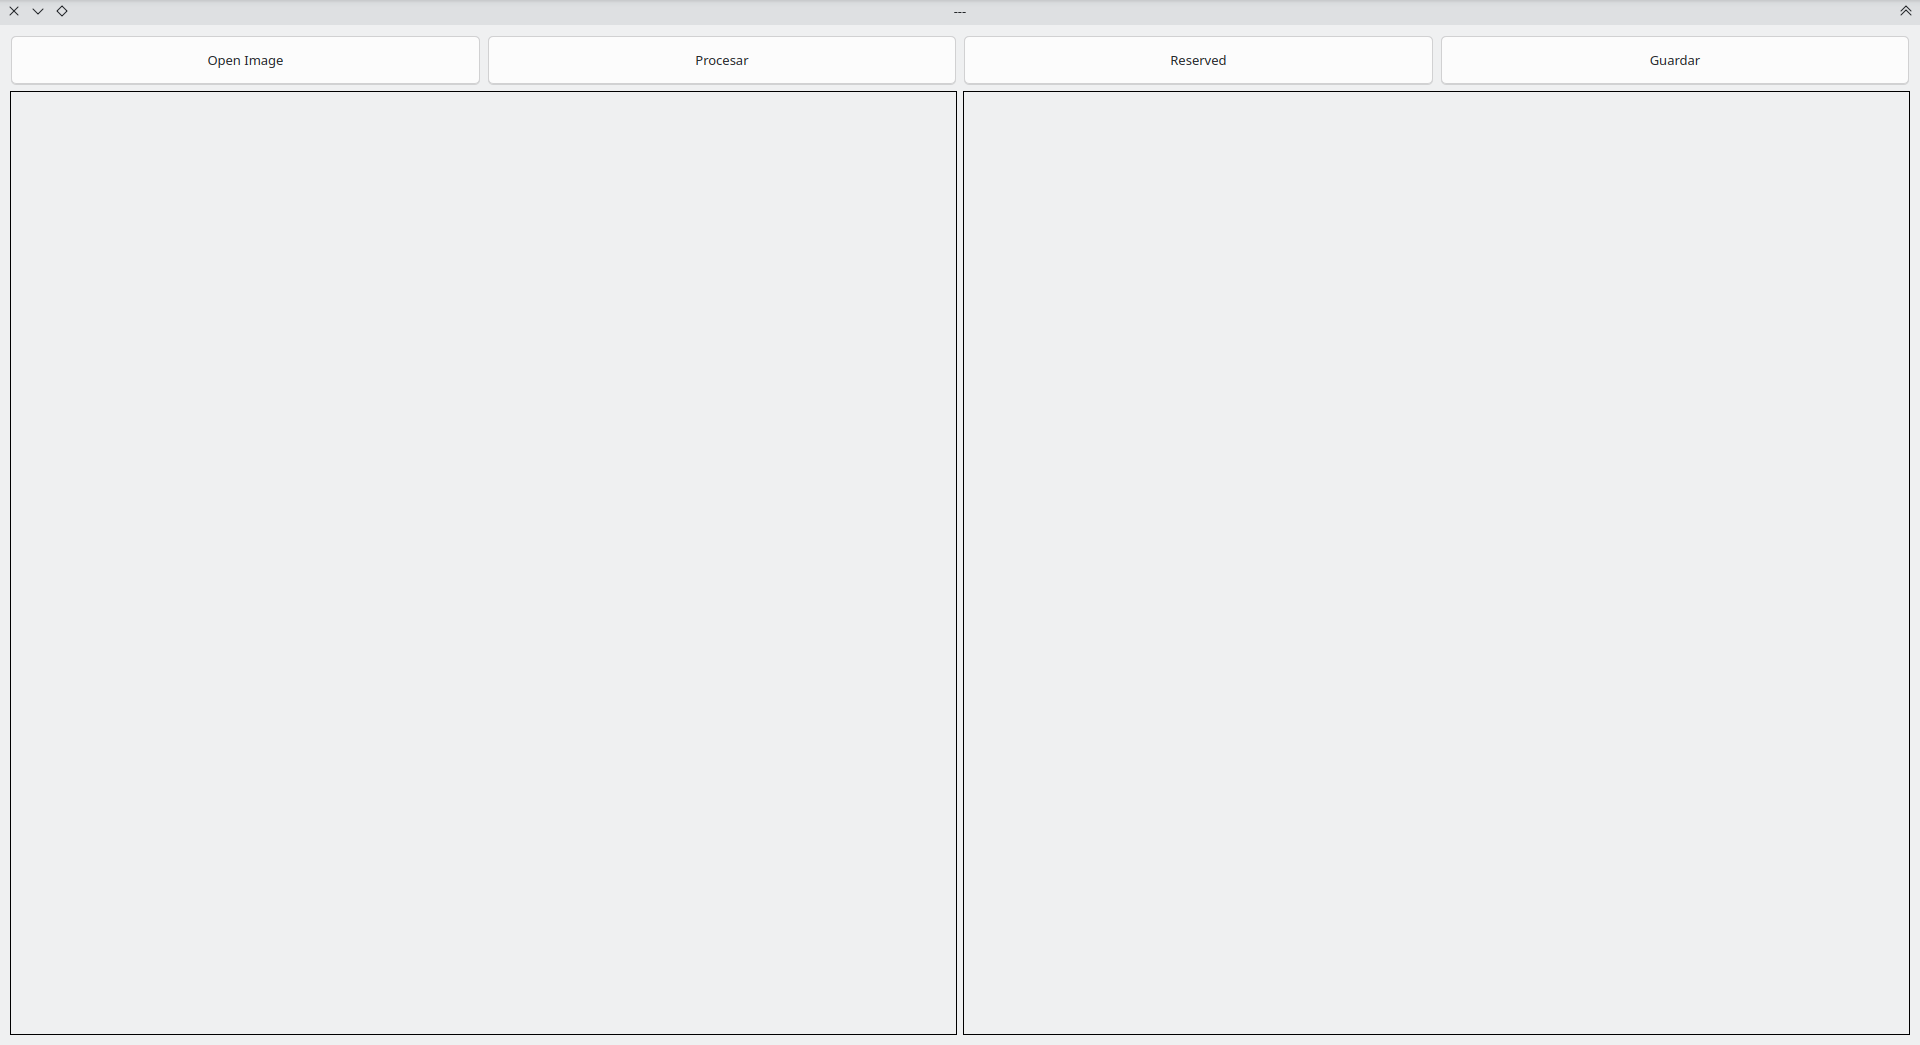
\includegraphics[width=\breite\linewidth]{images/UI.png}
        \caption{Interfaz del Sistema}
        \label{fig:res1}
    \end{figure}

    % images/pintos.png
    \begin{figure}[H]
        \centering
        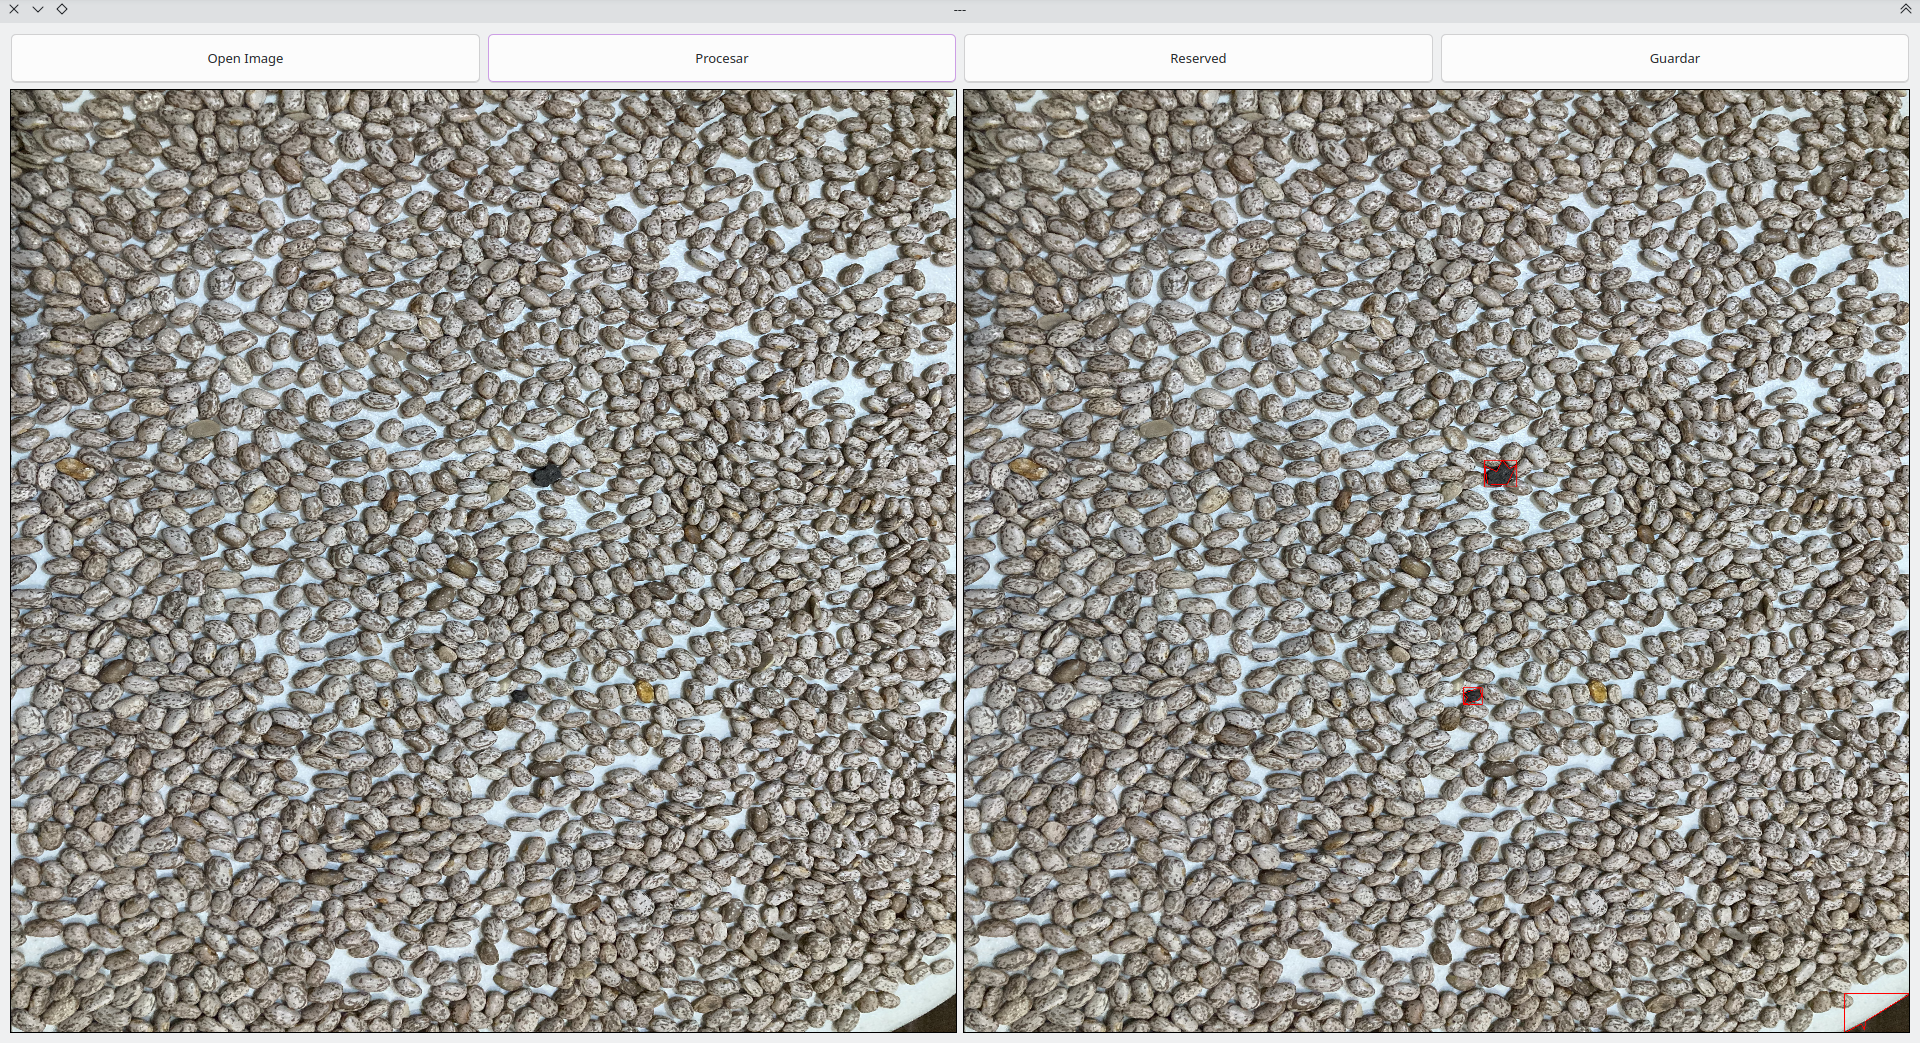
\includegraphics[width=\breite\linewidth]{images/pintos.png}
        \caption{}
        \label{fig:res2}
    \end{figure}

    % images/negros.png
    \begin{figure}[H]
        \centering
        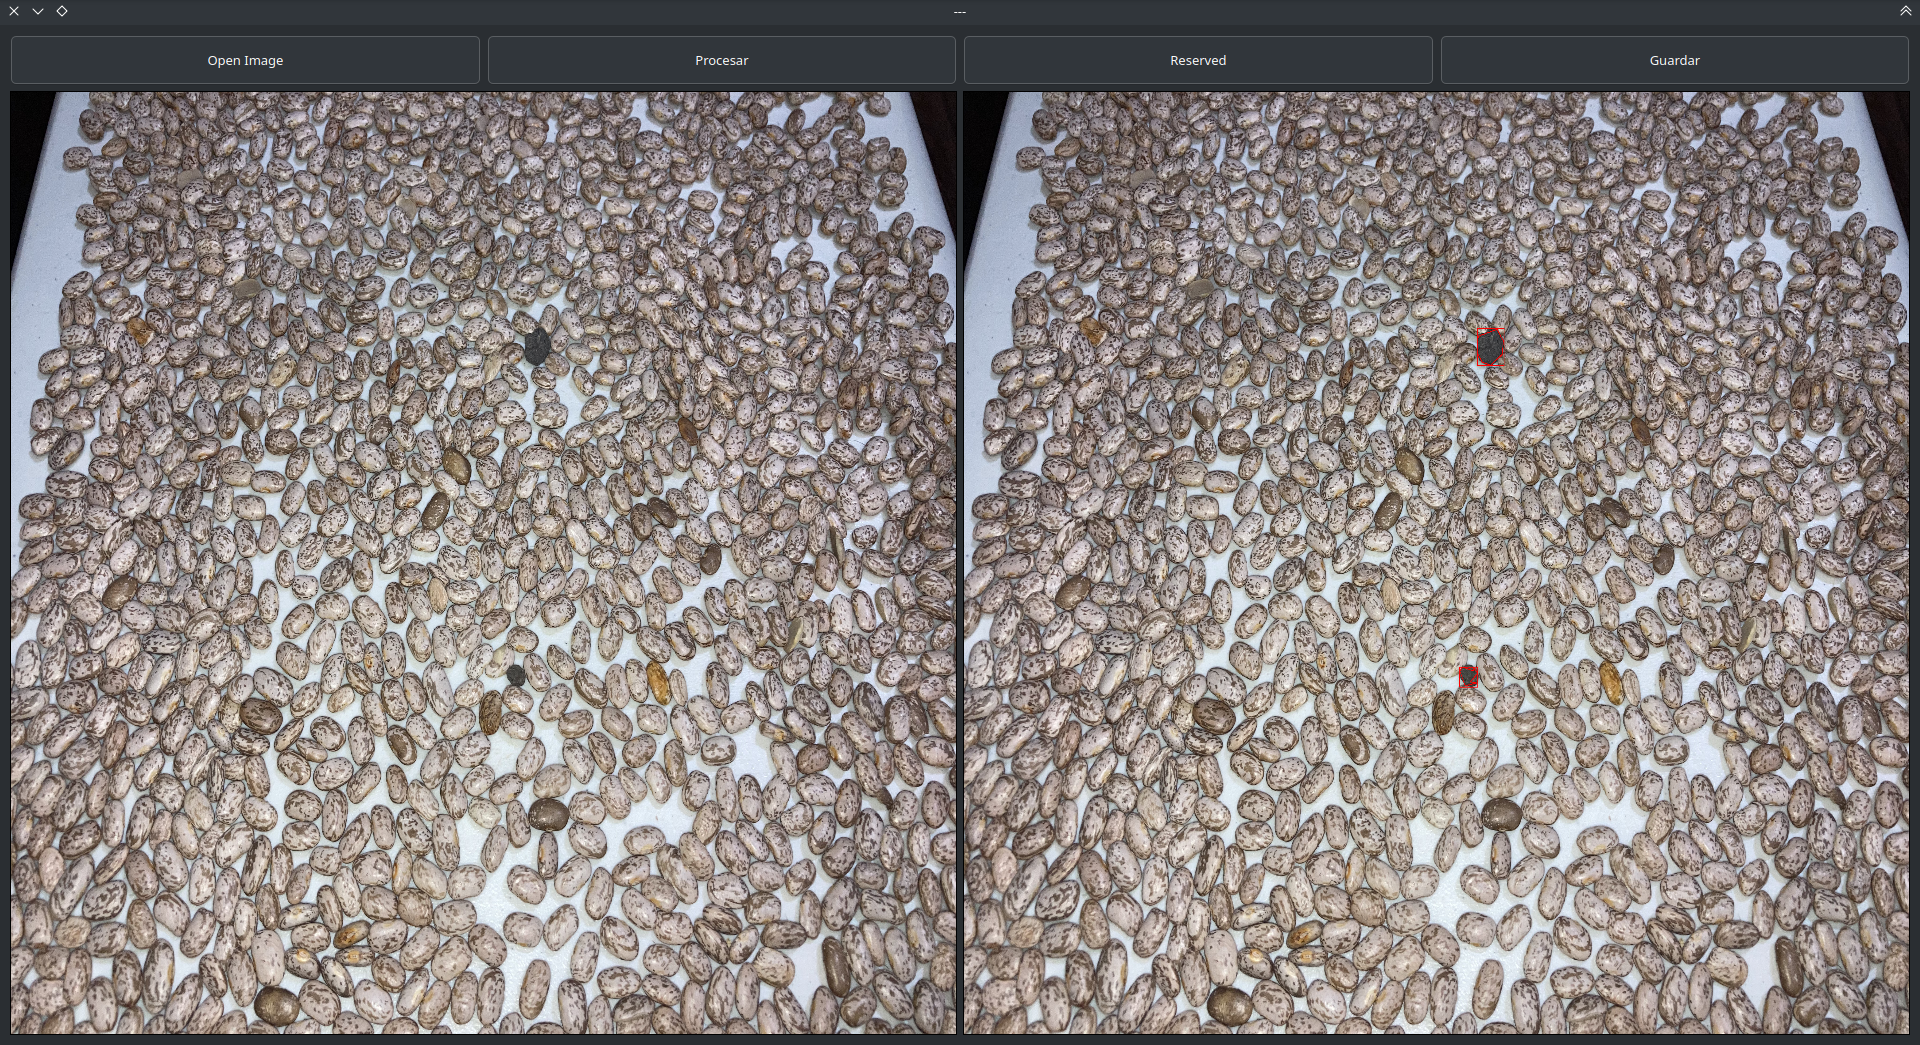
\includegraphics[width=\breite\linewidth]{images/negros.png}
        \caption{}
        \label{fig:res3}
    \end{figure}

    Los casos que se muestran son exitosos. A continuación se muestran las pruebas con imágenes nada controladas que incluso llegan a incumplir una calidad de imagen parecida a las imágenes que se probaron al realizar el programa, lo cual demuestra la baja robustez del sistema desarrollado.

    % test1.png
    \begin{figure}[H]
        \centering
        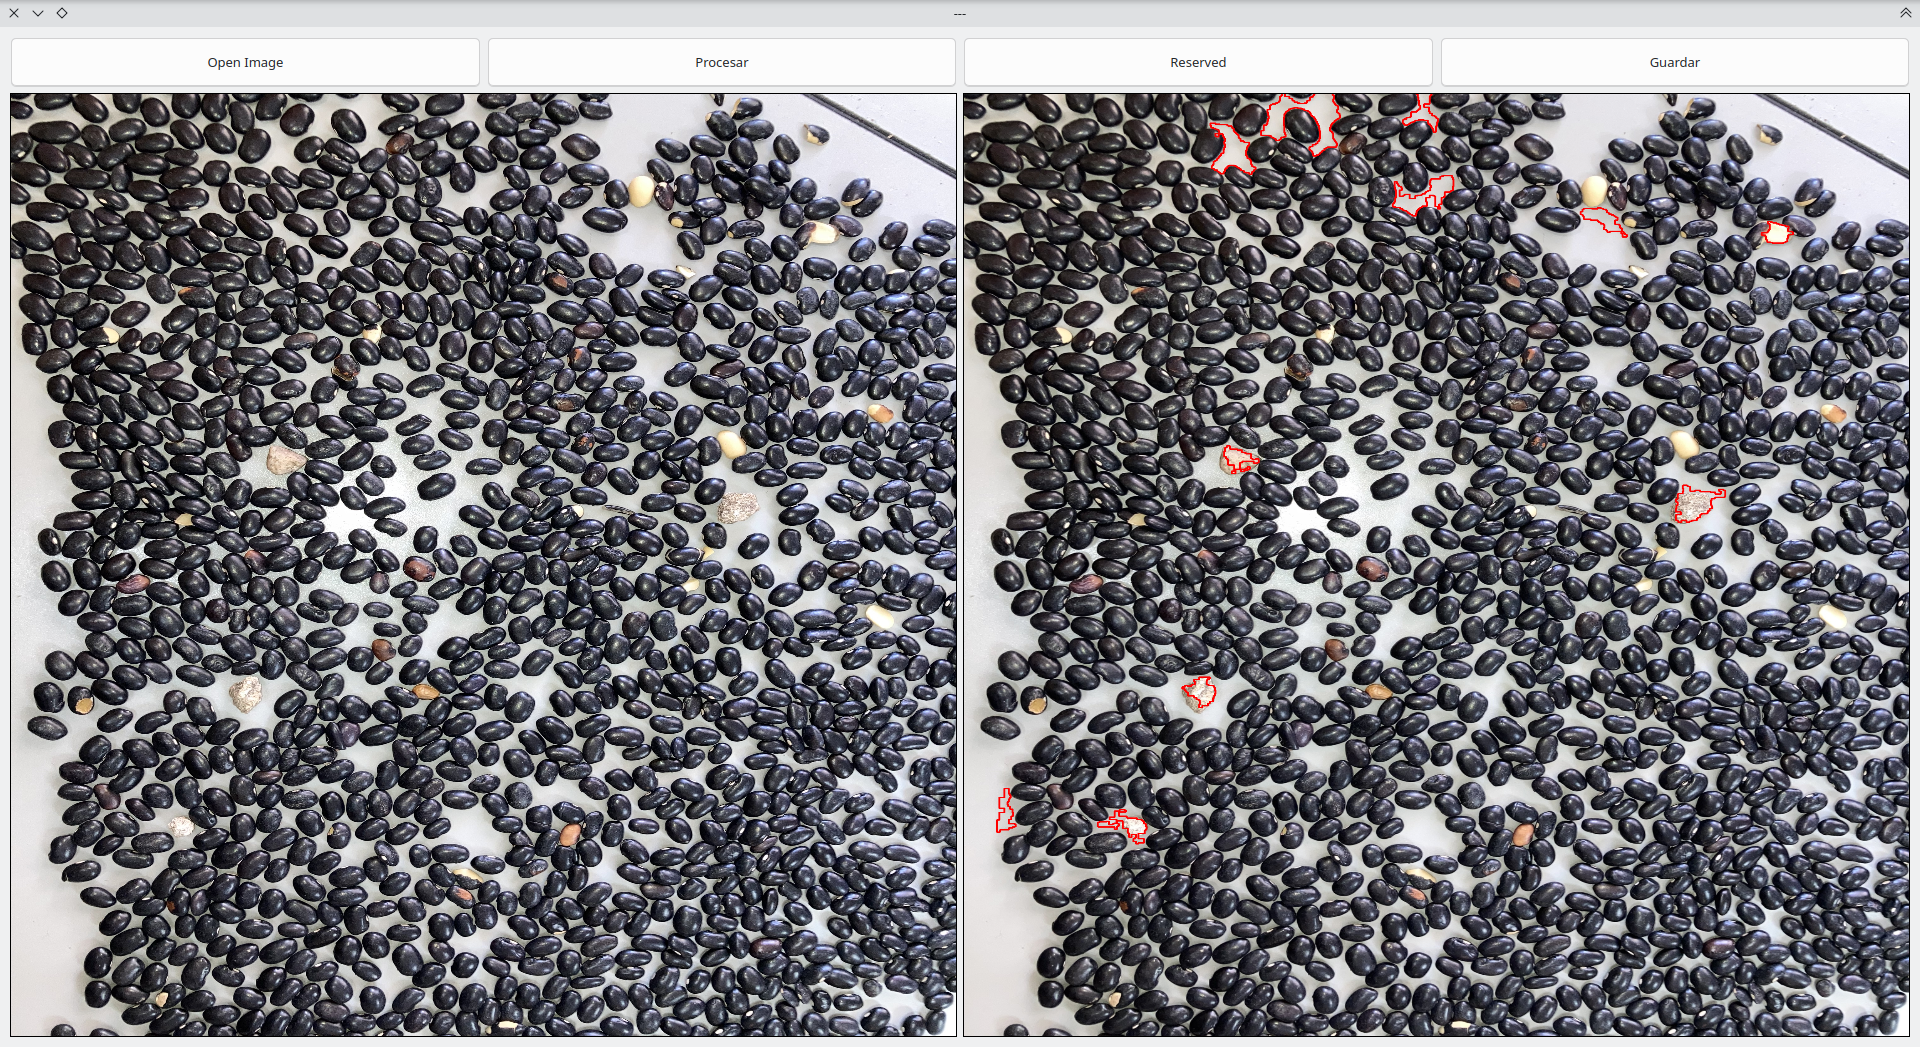
\includegraphics[width=\breite\linewidth]{images/test1.png}
        \caption{}
        \label{fig:test1}
    \end{figure}

    \begin{figure}[H]
        \centering
        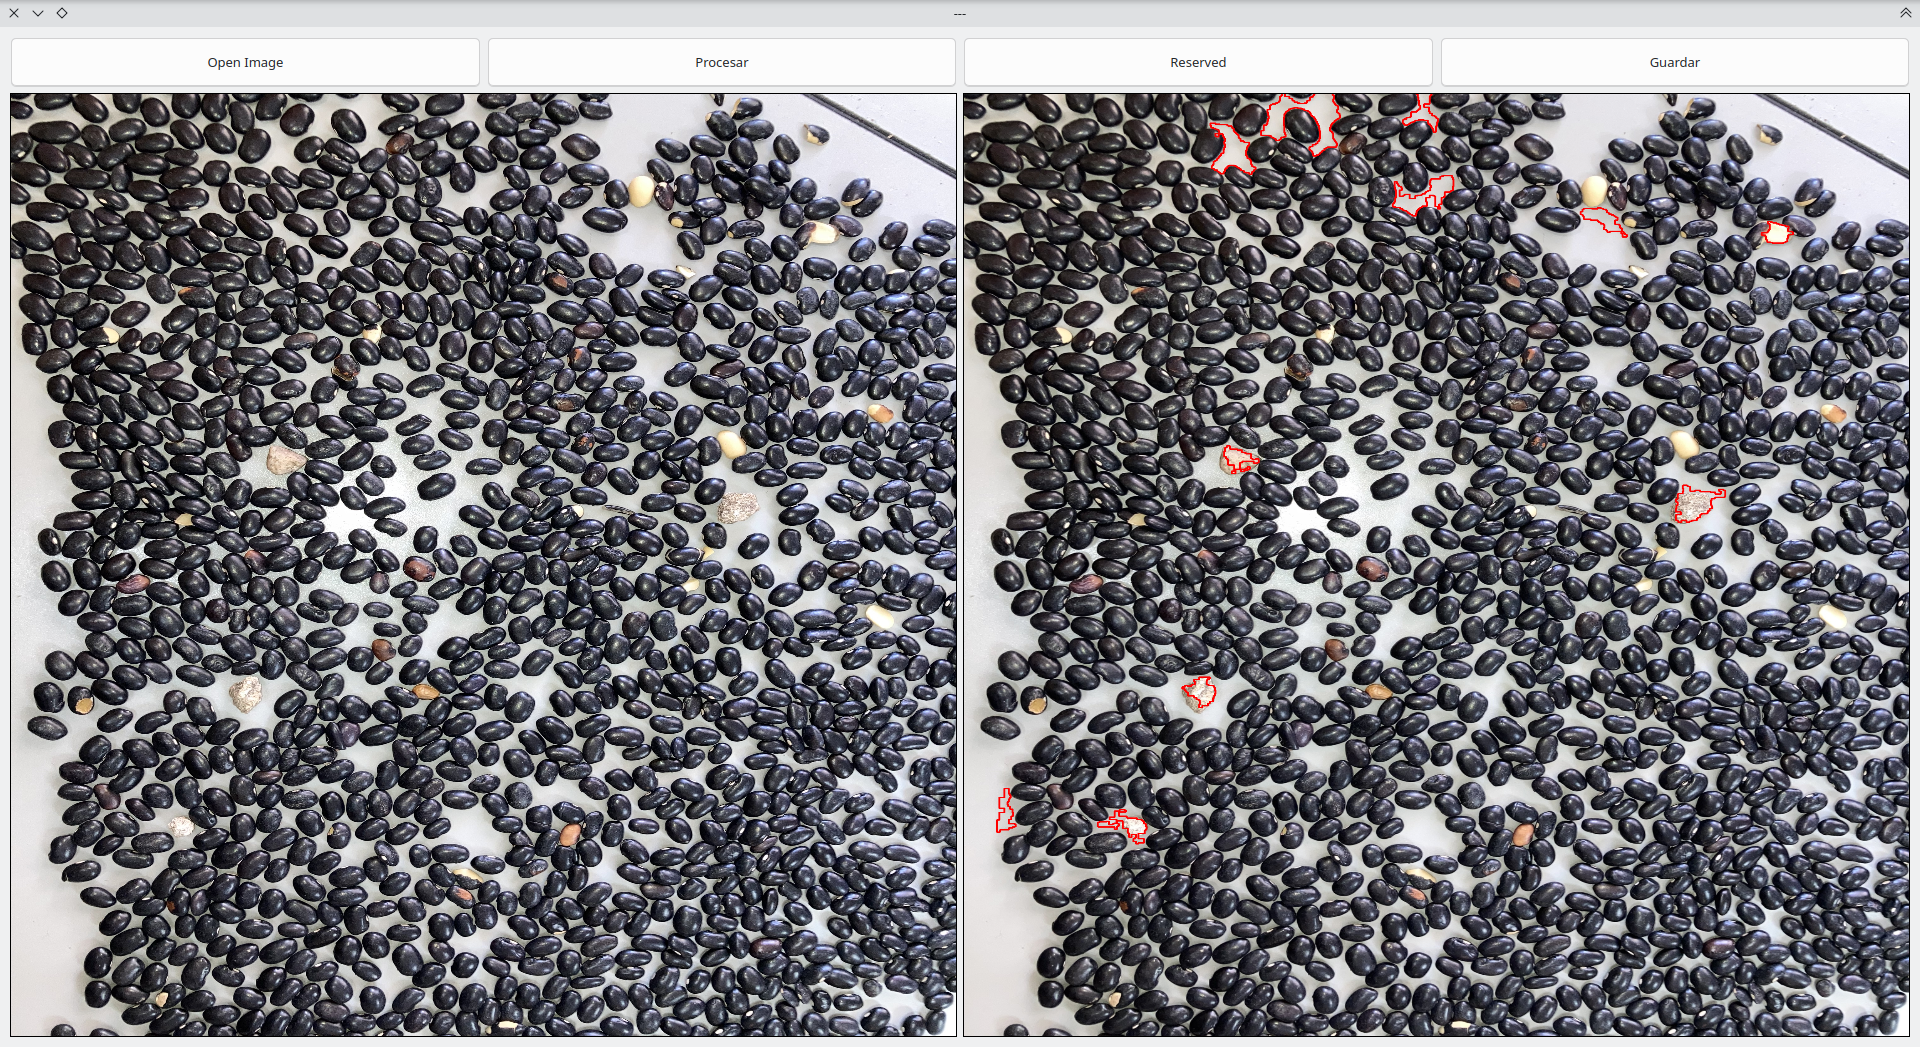
\includegraphics[width=\breite\linewidth]{images/test2.png}
        \caption{}
        \label{fig:test2}
    \end{figure}

    \begin{figure}[H]
        \centering
        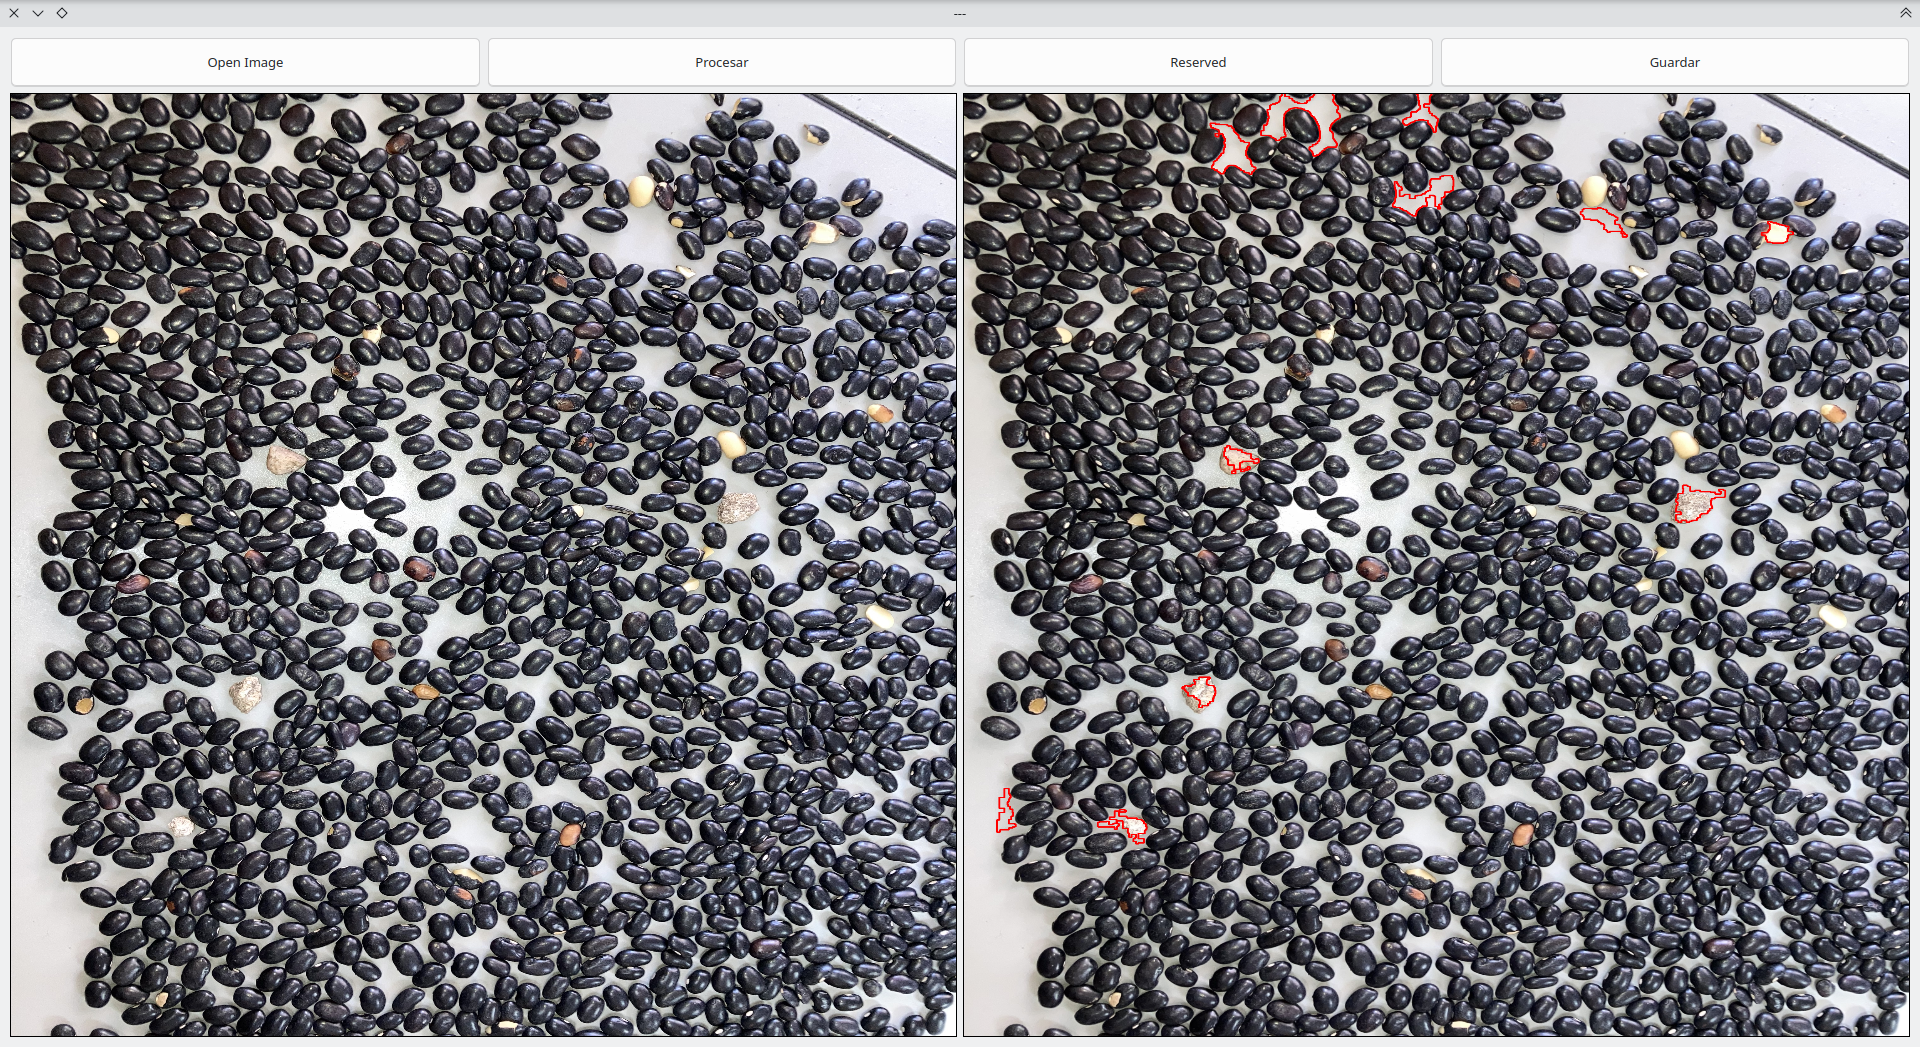
\includegraphics[width=\breite\linewidth]{images/test3.png}
        \caption{}
        \label{fig:test3}
    \end{figure}

    \begin{figure}[H]
        \centering
        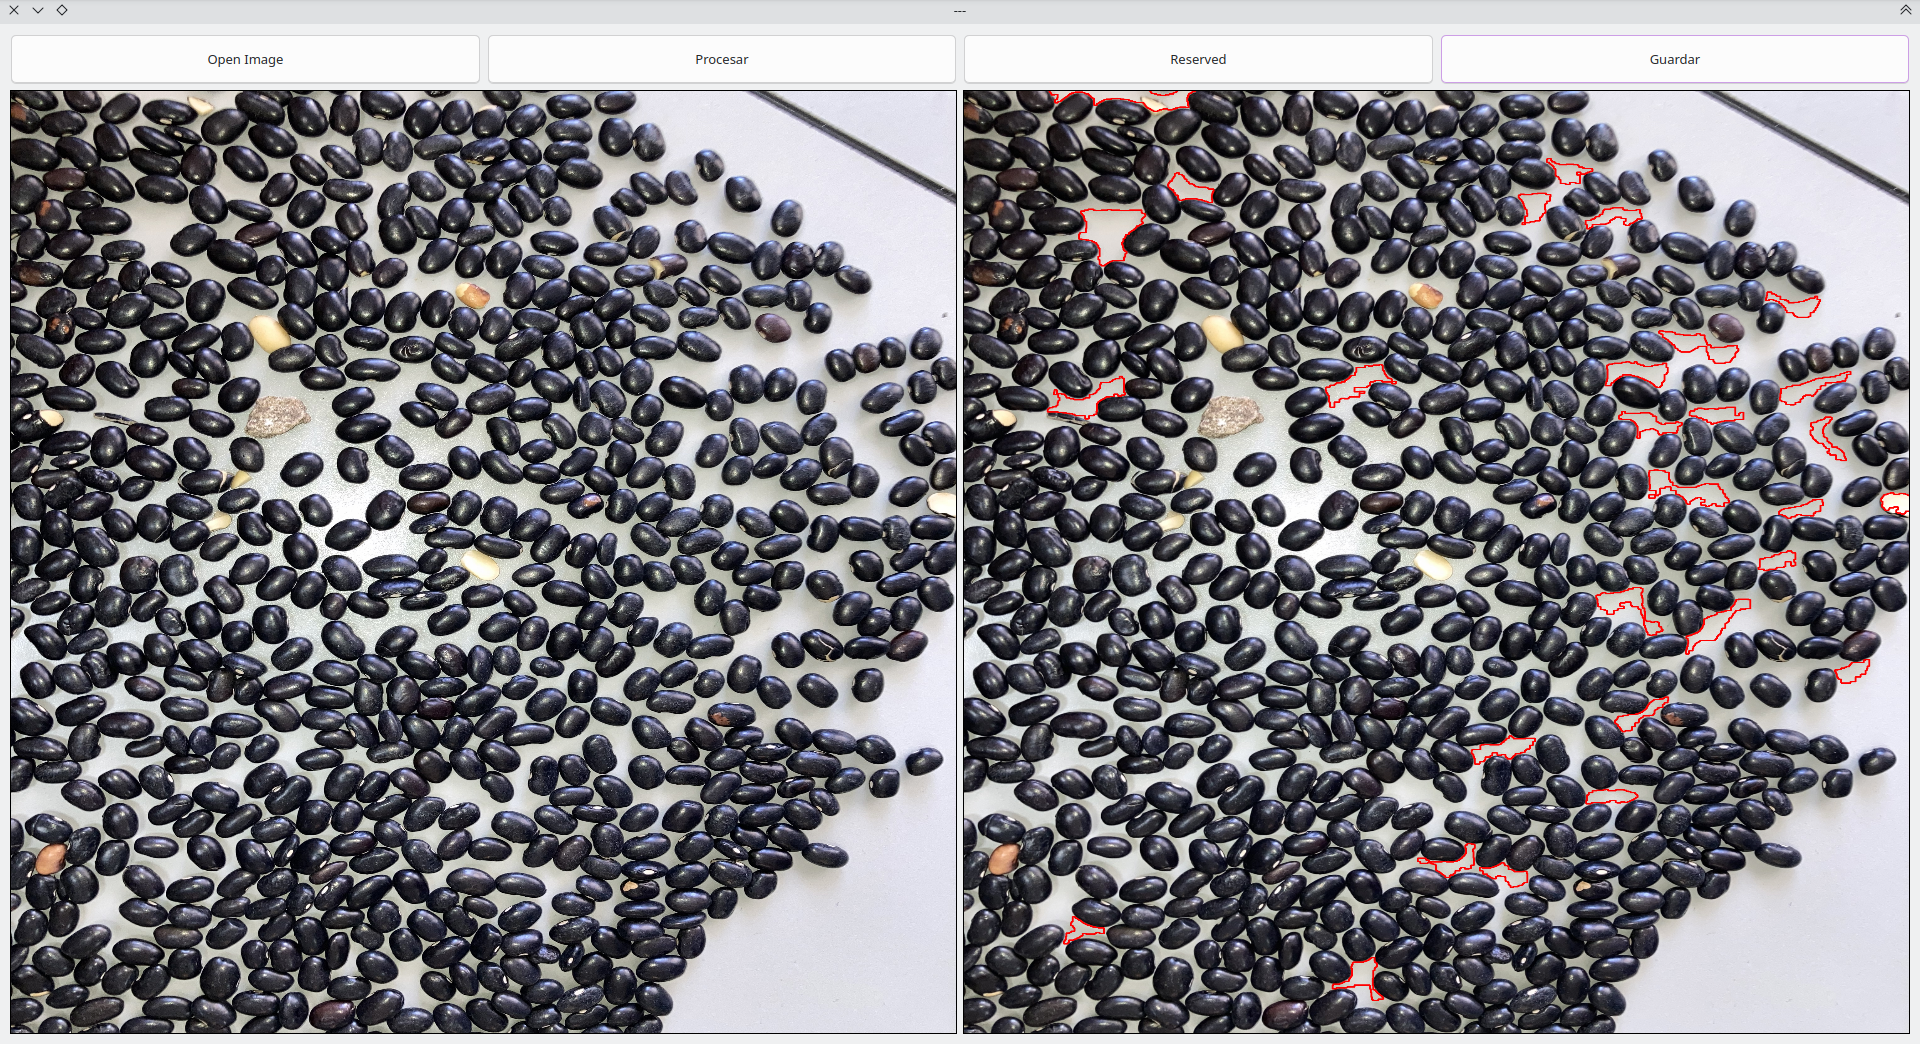
\includegraphics[width=\breite\linewidth]{images/test4.png}
        \caption{}
        \label{fig:test4}
    \end{figure}

    \begin{figure}[H]
        \centering
        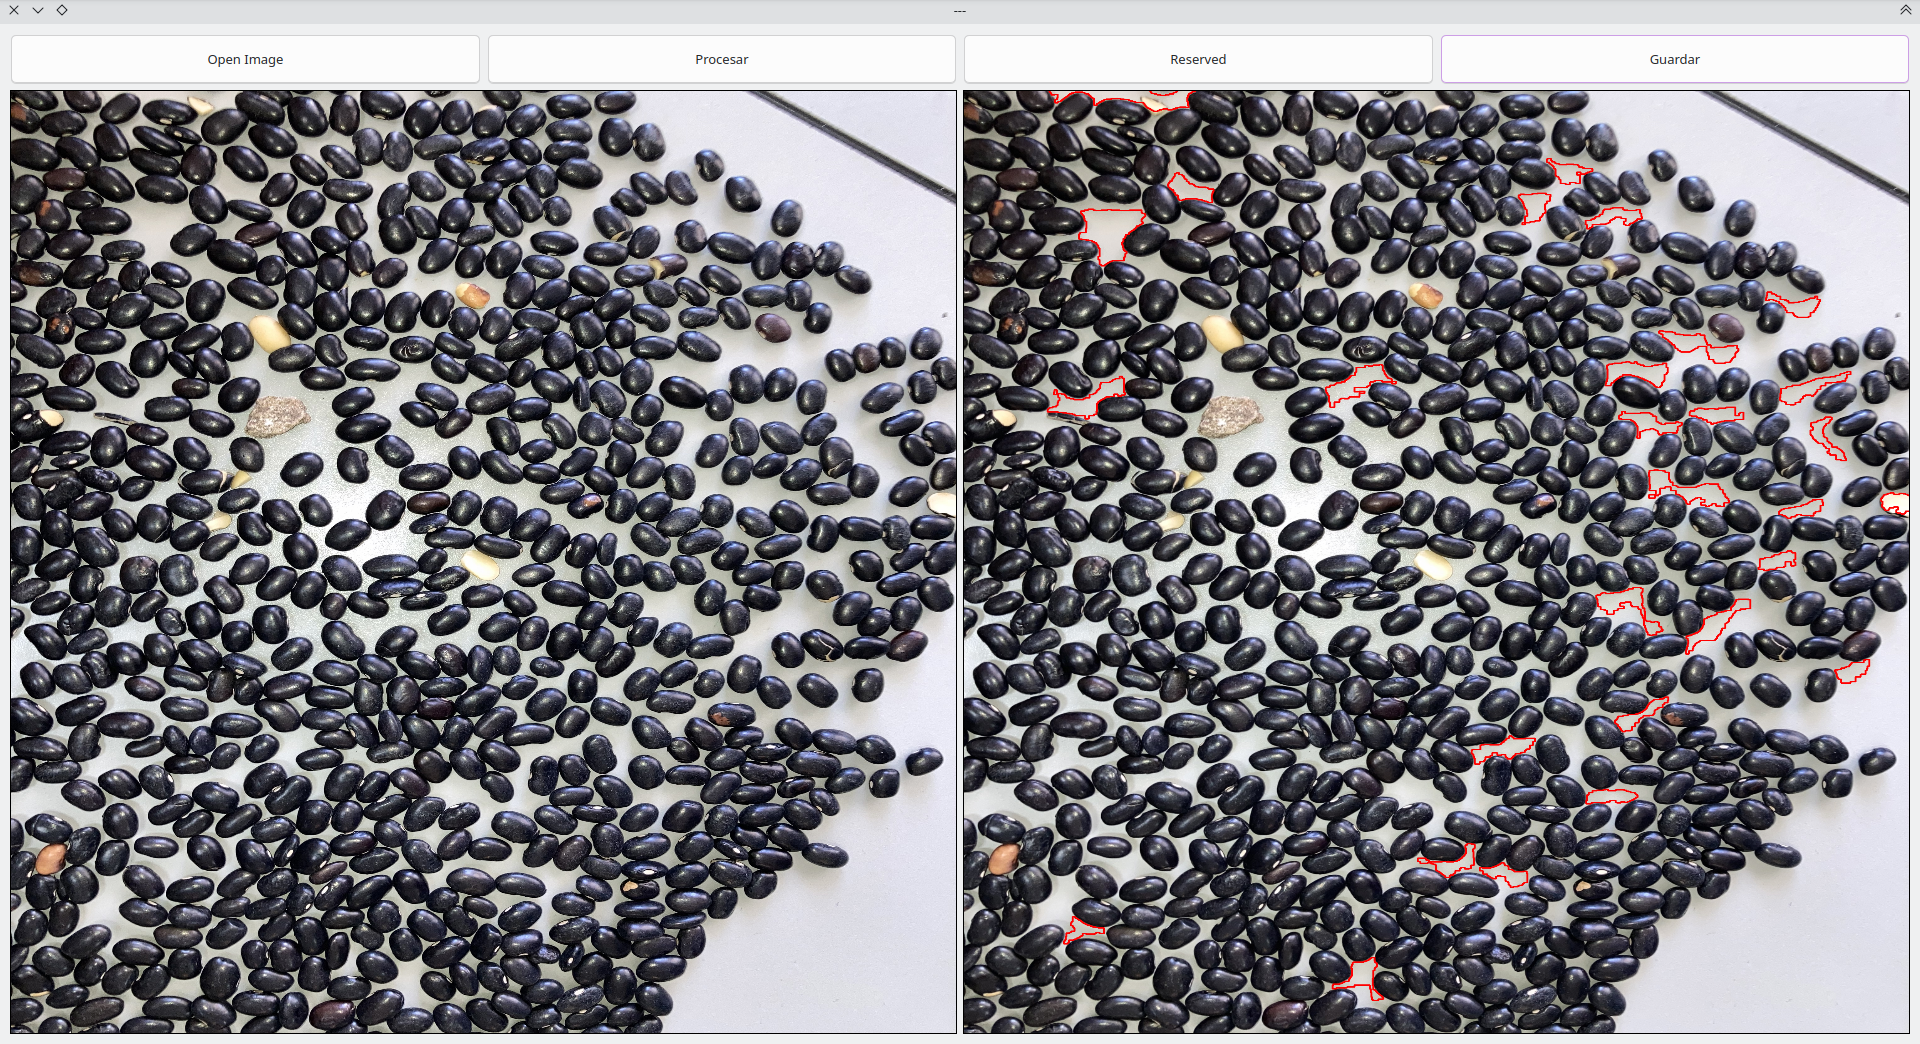
\includegraphics[width=\breite\linewidth]{images/test5.png}
        \caption{}
        \label{fig:test5}
    \end{figure}

    \begin{figure}[H]
        \centering
        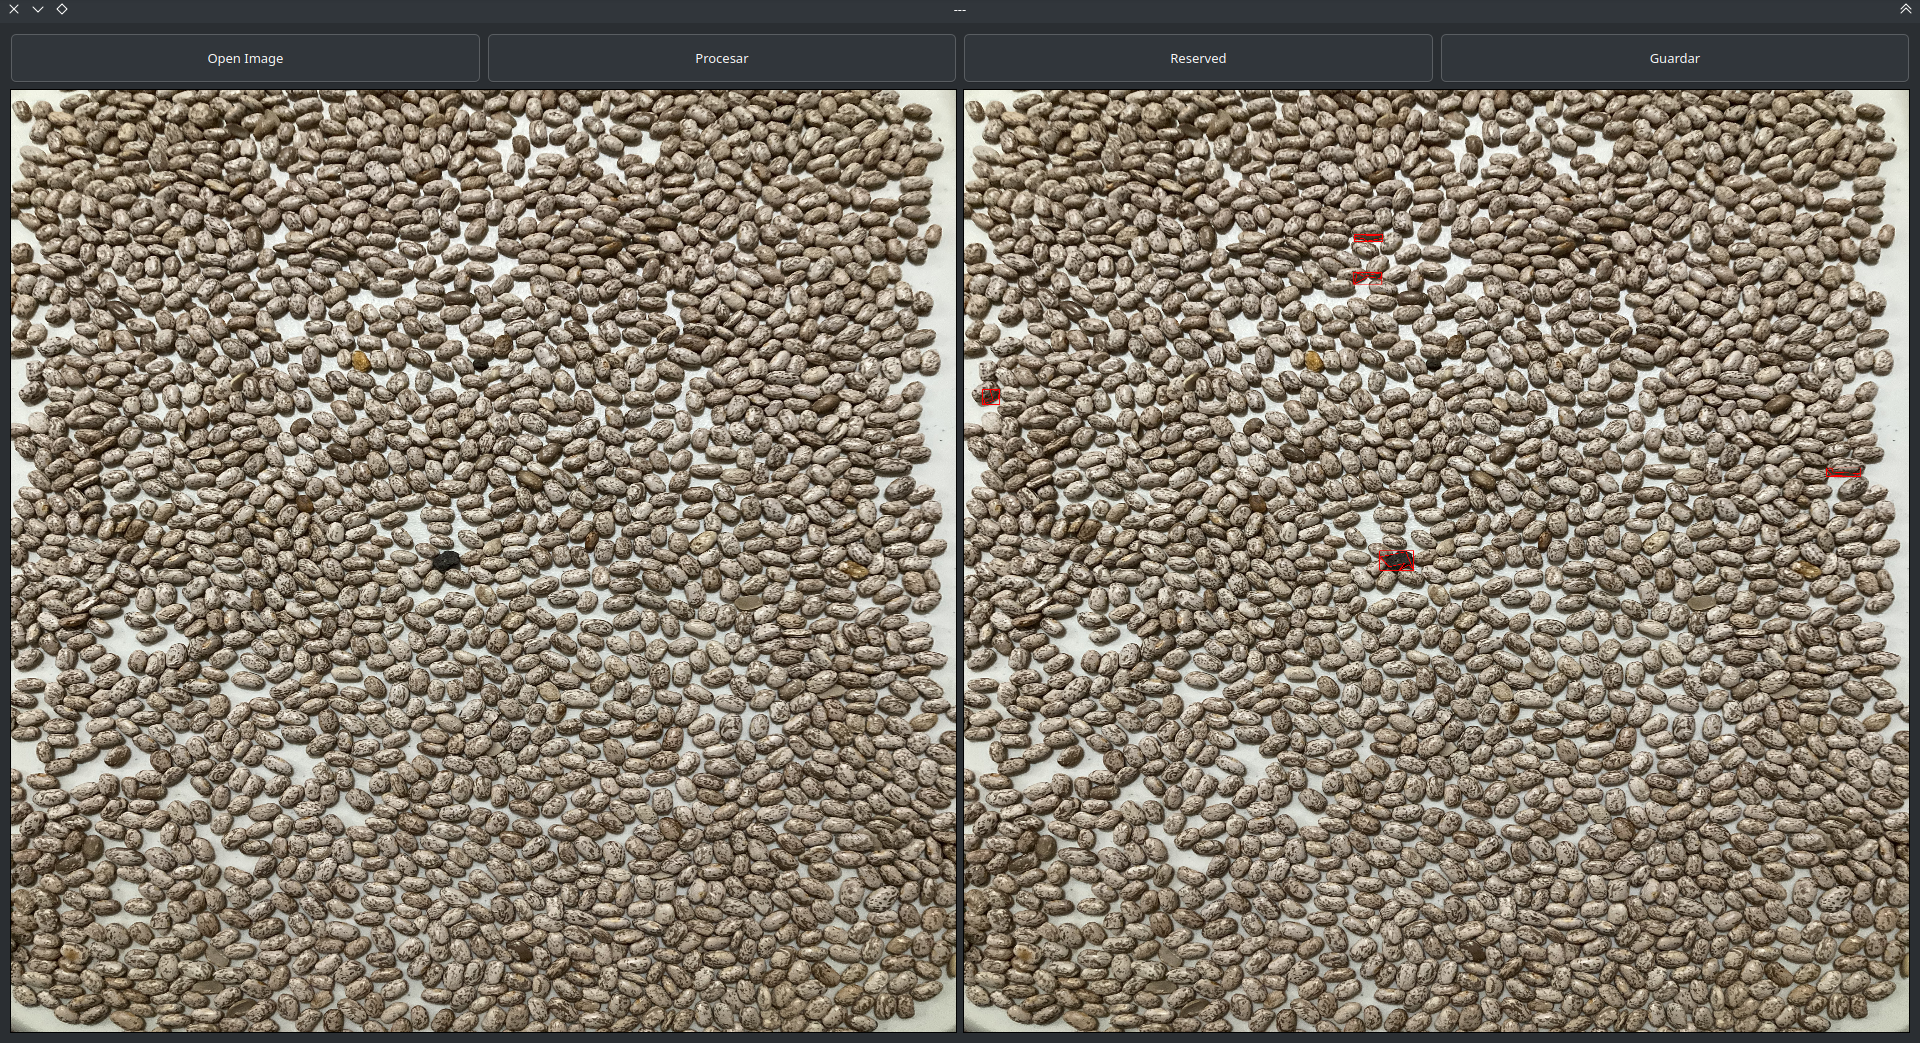
\includegraphics[width=\breite\linewidth]{images/test6.png}
        \caption{}
        \label{fig:test6}
    \end{figure}

    \begin{figure}[H]
        \centering
        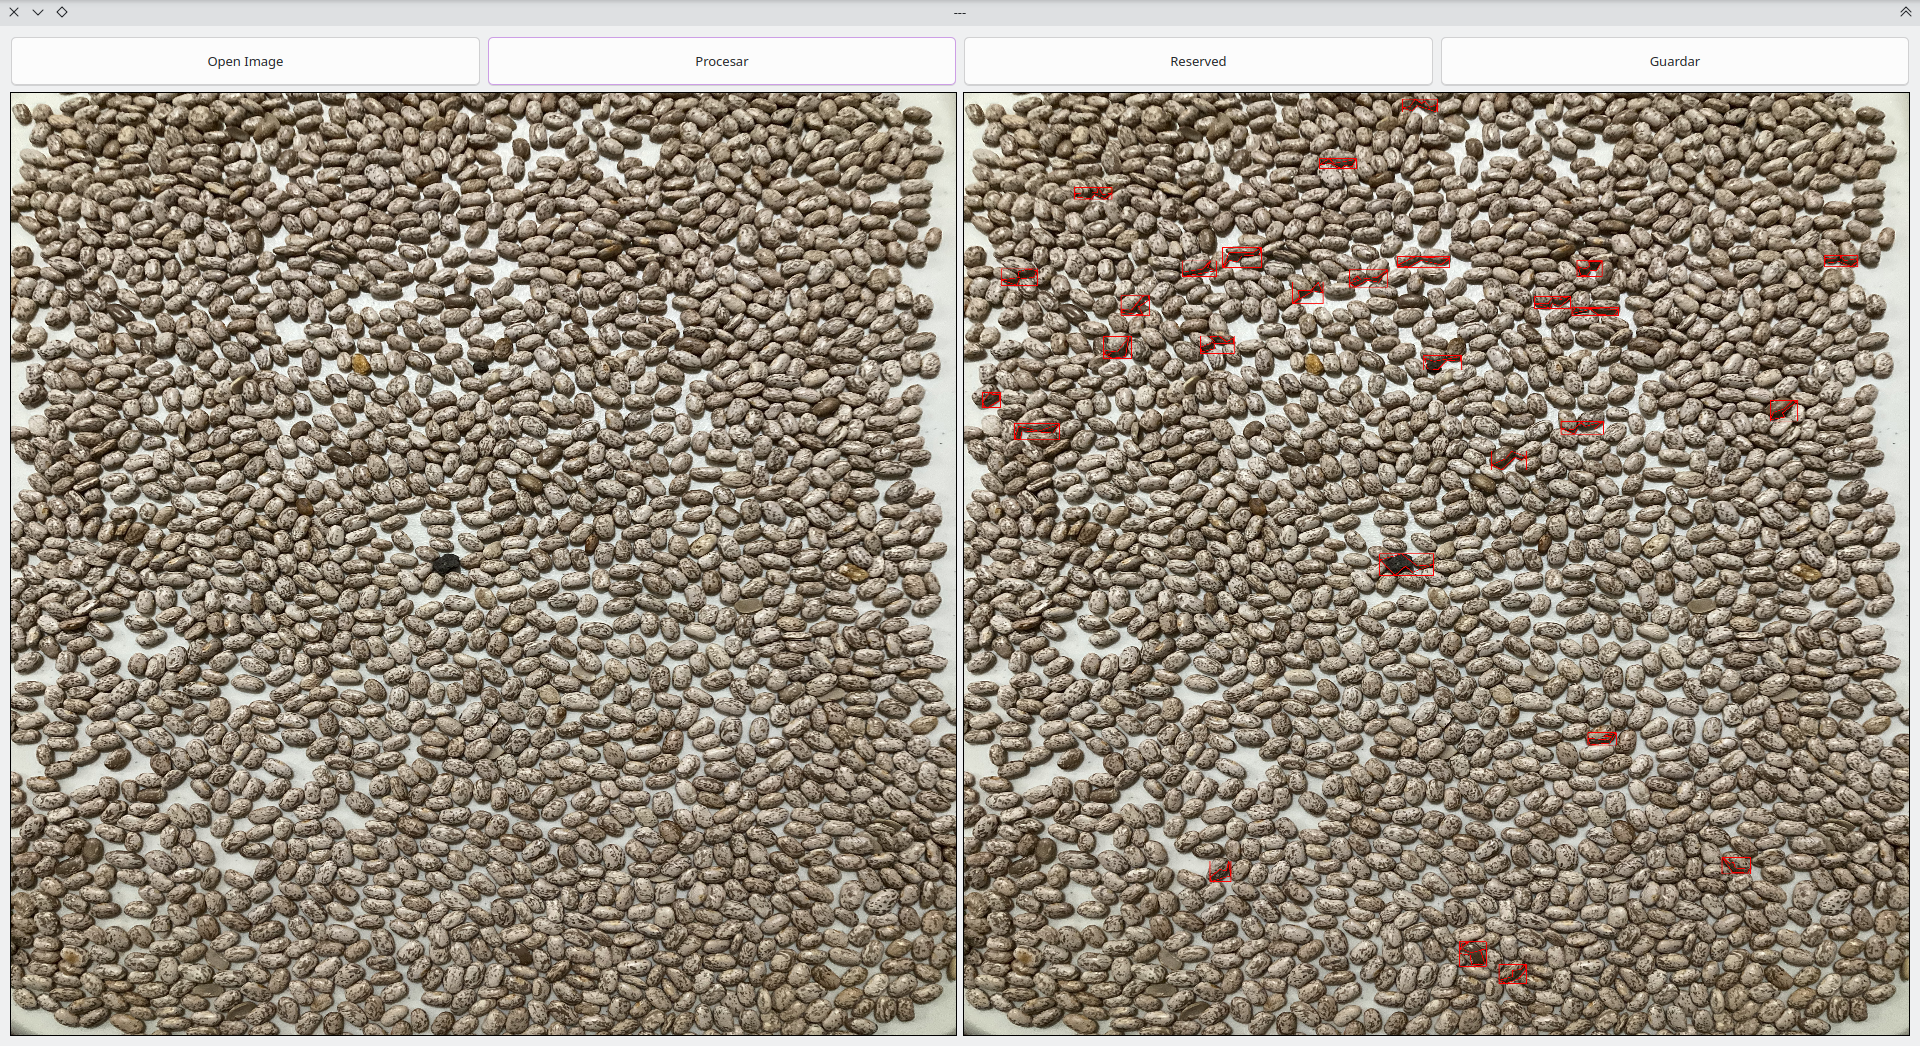
\includegraphics[width=\breite\linewidth]{images/test7.png}
        \caption{}
        \label{fig:test7}
    \end{figure}

    \begin{figure}[H]
        \centering
        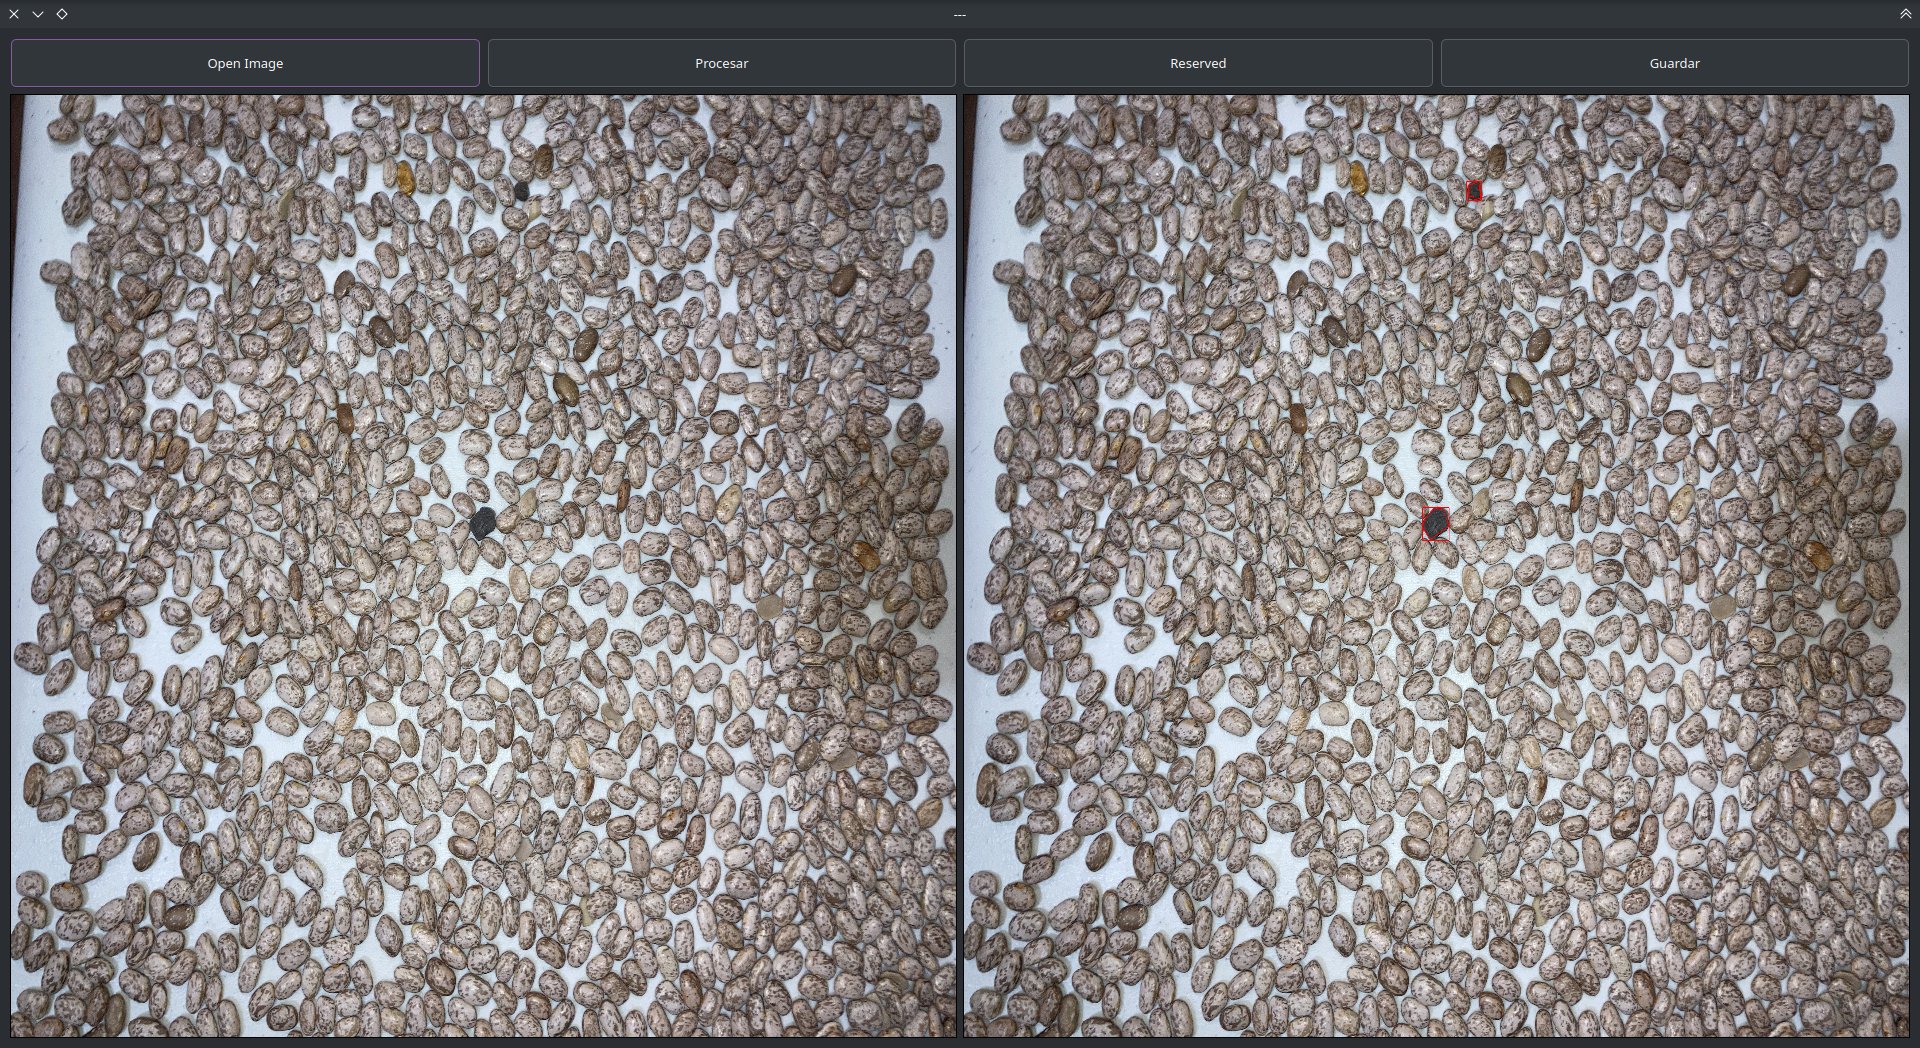
\includegraphics[width=\breite\linewidth]{images/test8.png}
        \caption{}
        \label{fig:test8}
    \end{figure}

    \begin{figure}[H]
        \centering
        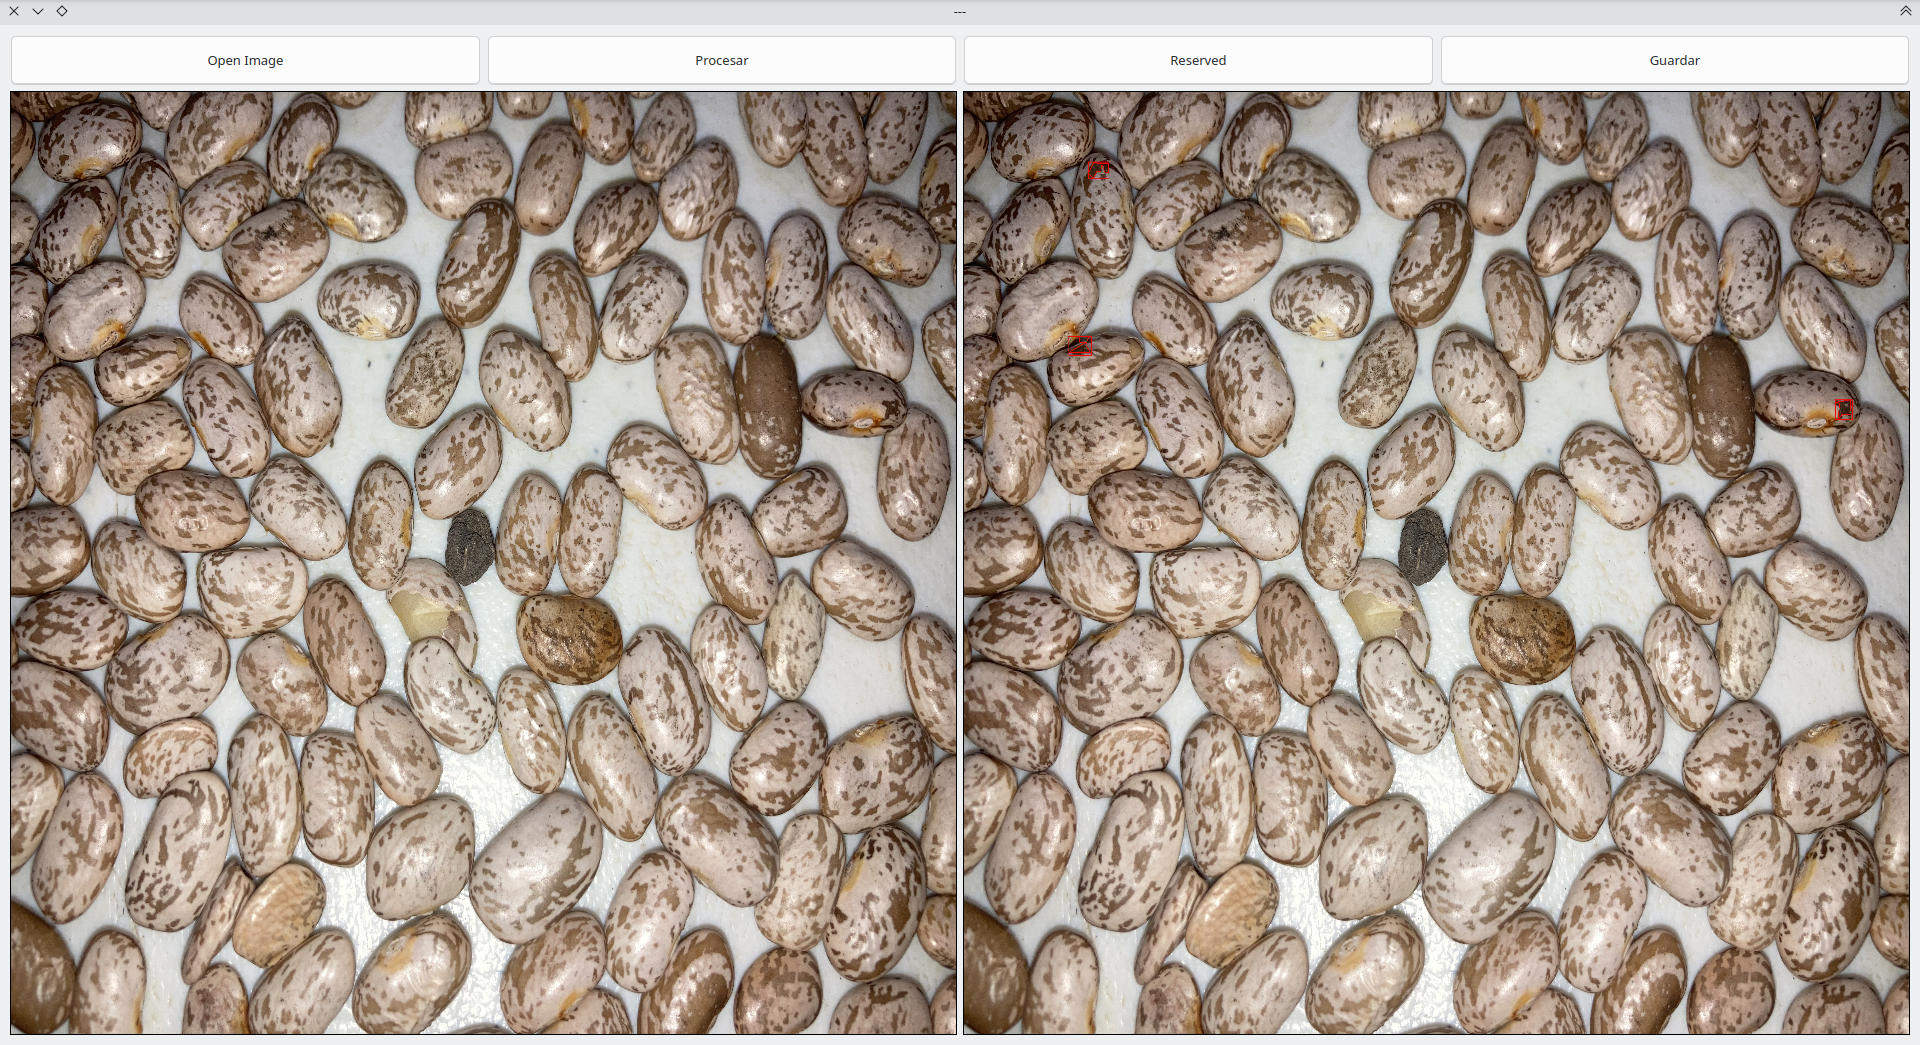
\includegraphics[width=\breite\linewidth]{images/test9.png}
        \caption{}
        \label{fig:test9}
    \end{figure}

    \begin{figure}[H]
        \centering
        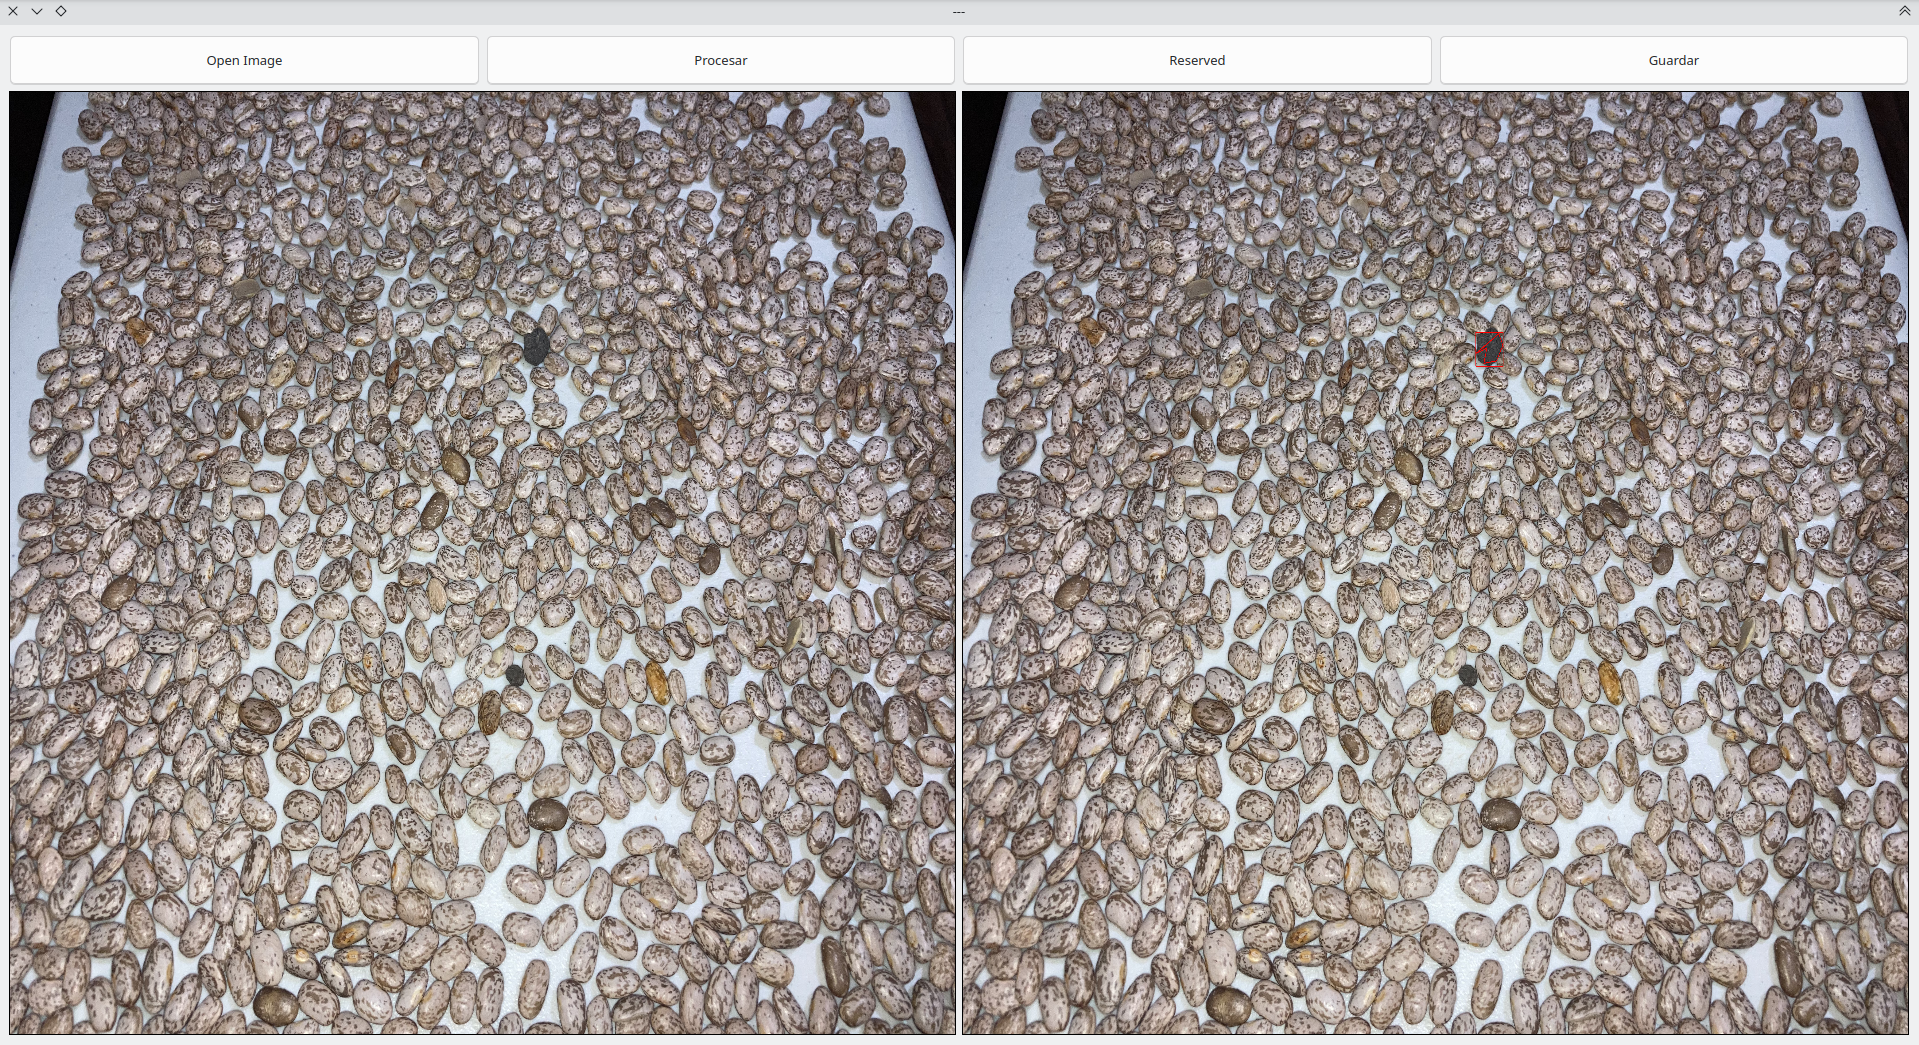
\includegraphics[width=\breite\linewidth]{images/test10.png}
        \caption{}
        \label{fig:test10}
    \end{figure}


%%%%%%%%%%%%%%%%%%%%%%%%%%%%%%%%%%%%%%%%%%%%%%%%%%%%%%%%%%%%%%%%%%%%%%%
\section{Conclusión}
    En este trabajo se propone un proyecto con la capacidad de detectar piedras entre un conjunto de frijoles usando solamente análisis de imágenes. Para lograr esto en palabras resumidas se usaron 2 características particulares de los frijoles la diferente convexidad que existe entre un frijol y una piedra, al igual que la diferencia del color. No se encontró algún proyecto en el cual podría inspirarse nuestro 

    A pesar de la nula experticia en el tema de análisis de imágenes por parte del equipo, el resultado fue funcional, mas simple; un sistema con cierta cantidad de asertividad, mas no con la suficiente robustez.
    

%%%%%%%%%%%%%%%%%%%%%%%%%%%%%%%%%%%%%%%%%%%%%%%%%%%%%%%%%%%%%%%%%%%%%%%
\nocite{*}
\addcontentsline{toc}{section}{Referencias} 
\printbibliography
%\balance

\end{document}